\section{Data Model}
\label{sec:dm}

The data model brings together environmental records that differ in subject,
identifier and reporting grain. It is the outcome of the integration and
normalization work described in Section~\ref{sec:norm}. Reference relations
identify stations, districts, rivers and categories; time relations distinguish
calendar and fiscal periods; observation relations store one defined fact type
at one declared grain. This structure keeps the data queryable without forcing
daily, monthly, yearly and fiscal records into one general-purpose table.

\subsection{Approved Final Entity--Relationship Diagram}
\label{subsec:erd}

Figure~\ref{fig:final-erd} is the approved final ERD used by the SQLite
implementation, normalization outputs and this report. It is the same Group-07
diagram retained in the earlier report versions. No ERD evolution sequence is
shown because the report does not have a complete, verified set of intermediate
diagrams. The editable source is available through the
\href{https://excalidraw.com/#json=j3fisE2kuM0i3LrmglI5T,IdqA_wfX0o7rkb26N7PfFw}
{Group-07 final ERD in Excalidraw}.

The diagram can be read in three layers. Reference and time relations provide
the reusable identifiers, observation relations store the measurements, and
foreign-key paths connect each measurement to its available place, period or
category. Table~\ref{tab:erd-reading-guide} gives a compact guide before the
full-page drawing.

\begin{table}[H]
\centering
\caption{Reading guide for the approved final ERD}
\label{tab:erd-reading-guide}
\begin{tabular}{L{0.22\textwidth}L{0.33\textwidth}L{0.35\textwidth}}
\toprule
Relation family & Examples & Role in the model \\
\midrule
Reference & \texttt{Station}, \texttt{District}, \texttt{River},
\texttt{Size}, \texttt{Industry\_Type} & Reusable place and category values. \\
Time & \texttt{Year\_Time}, \texttt{Month\_Time}, \texttt{Day\_Time},
\texttt{Fiscal\_Year} & Valid calendar and fiscal-period combinations. \\
Observation & Climate, water-quality, forest and industrial relations & Facts
stored at their published monthly, daily, yearly or fiscal grain. \\
\bottomrule
\end{tabular}
\end{table}

\clearpage
\newgeometry{hmargin=0.4in,vmargin=0.8in}
\begin{landscape}
\thispagestyle{plain}
\begin{figure}[H]
\centering
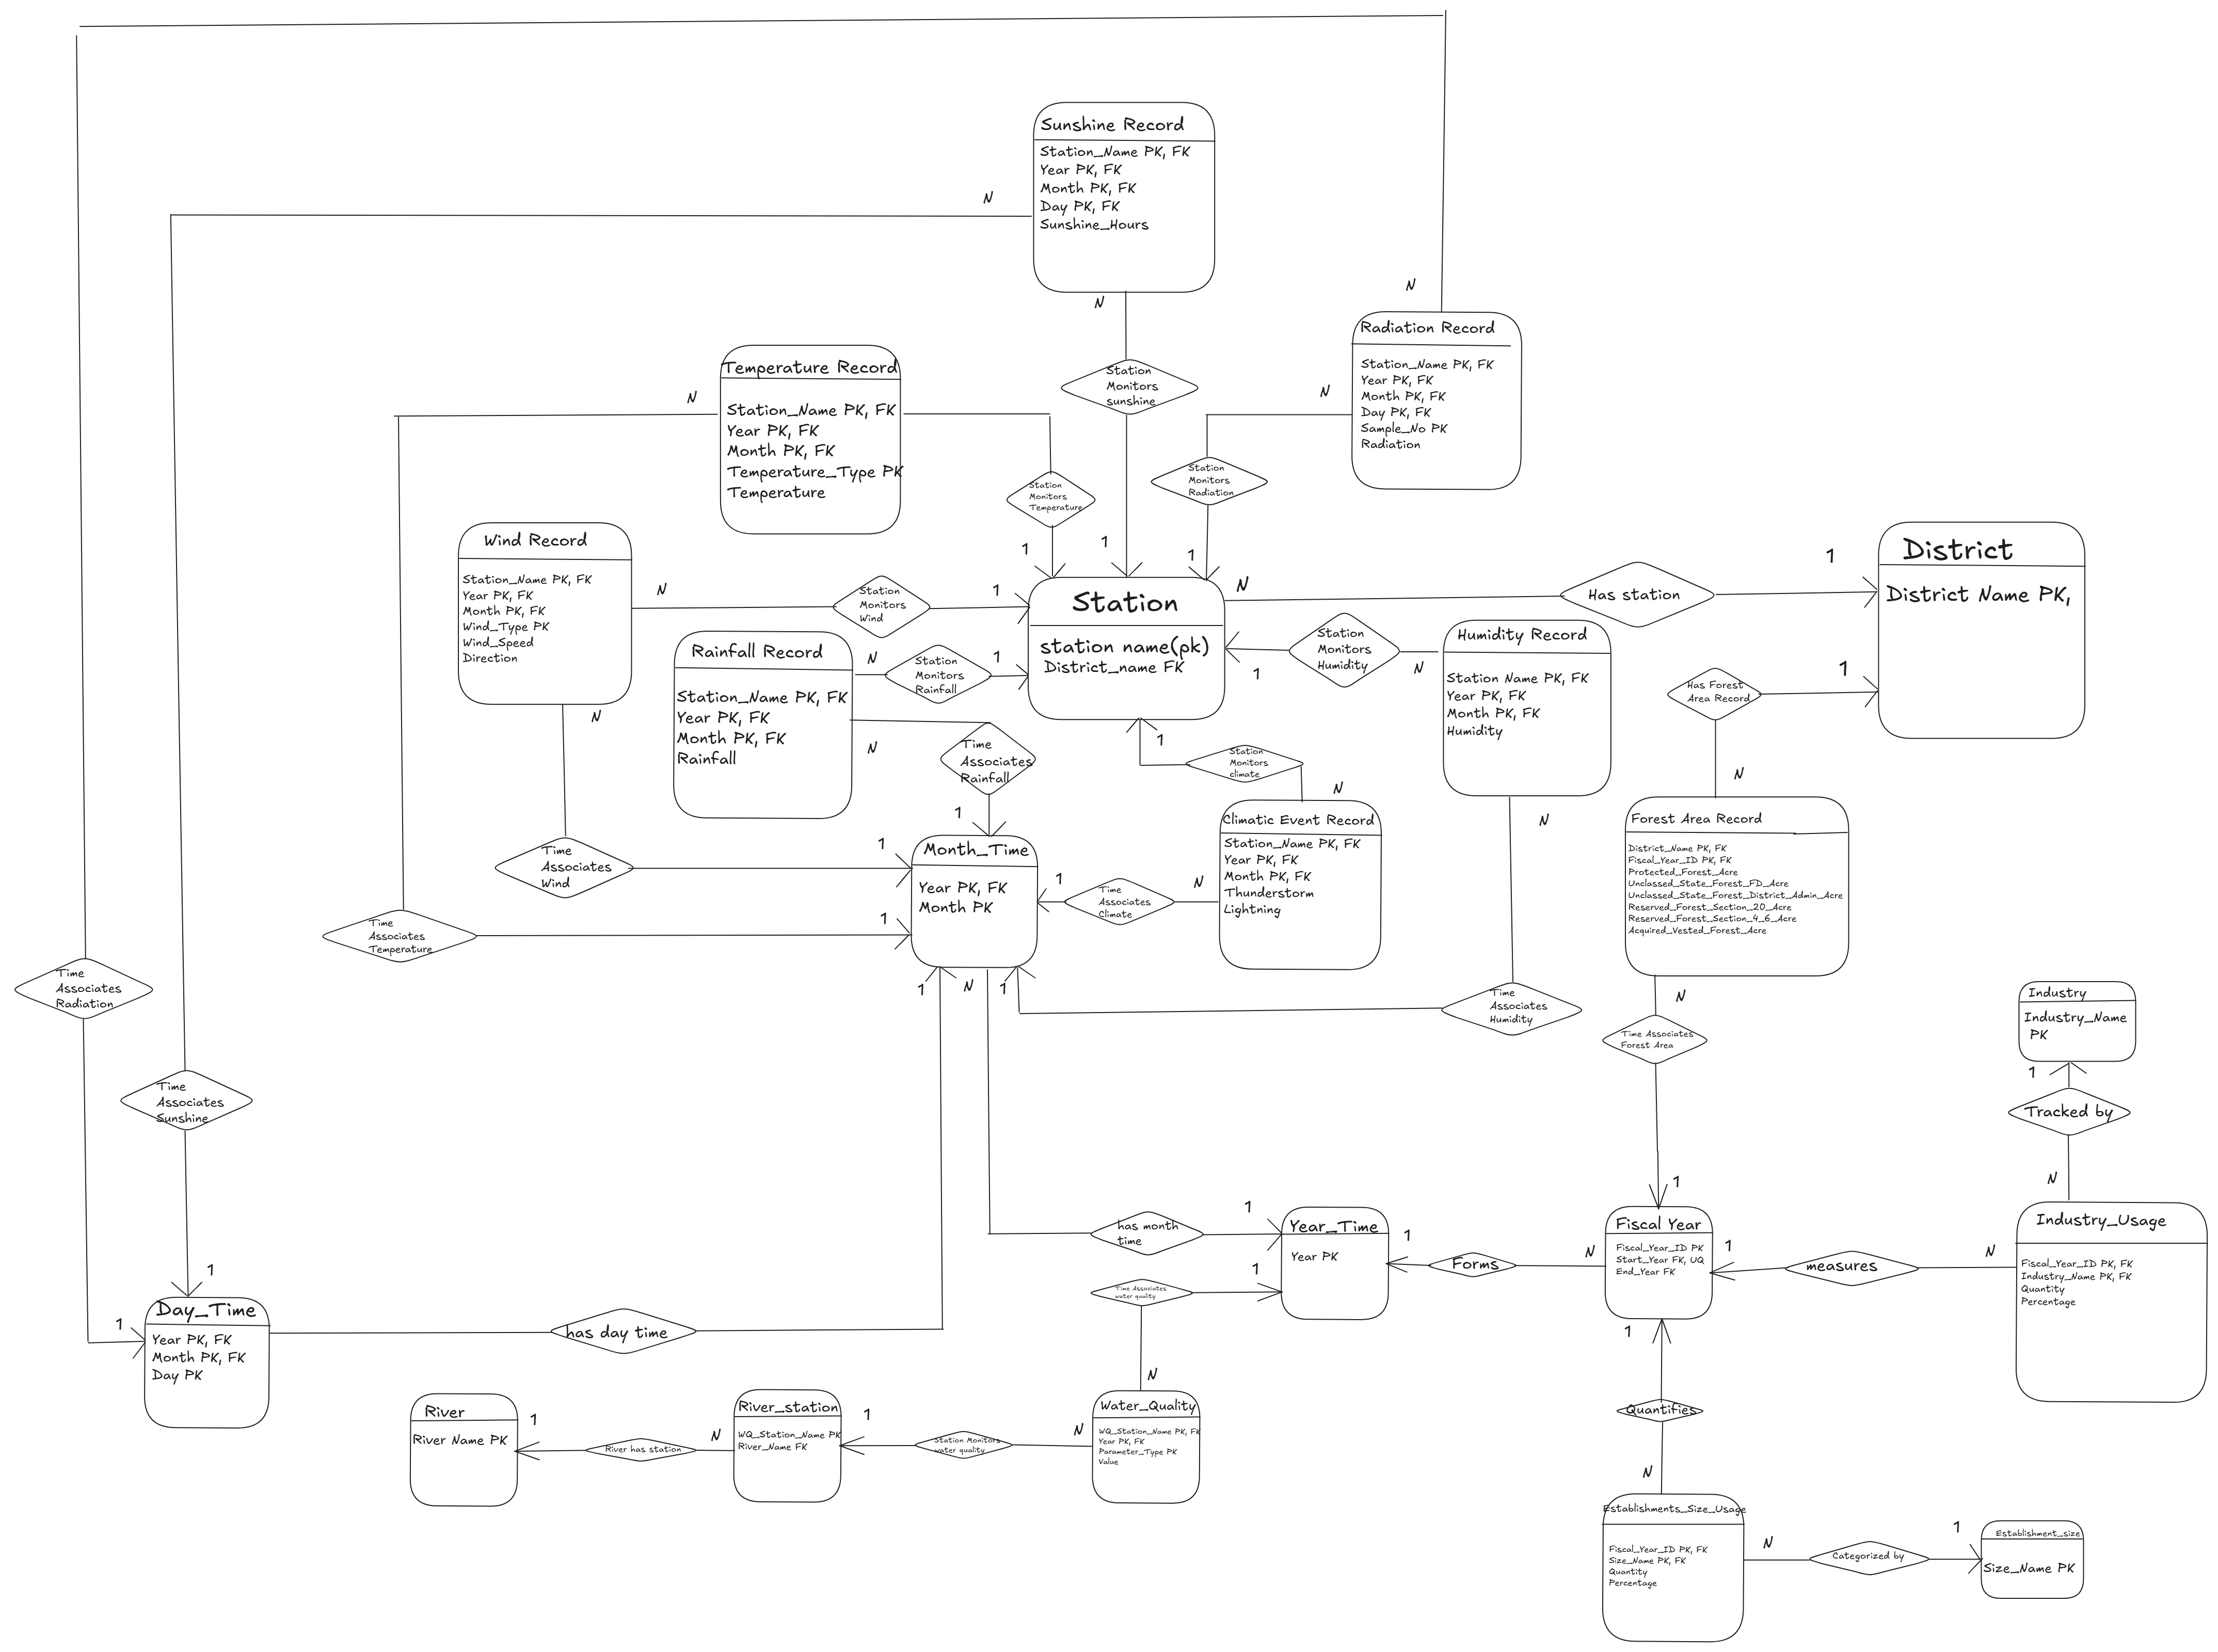
\includegraphics[width=\linewidth,height=0.90\textheight,keepaspectratio]
  {Final_erd.png}
\caption{Approved final Group-07 environmental ERD in BCNF. Source: the
linked Group-07 Excalidraw drawing.}
\label{fig:final-erd}
\end{figure}
\end{landscape}
\restoregeometry
\clearpage

\subsection{Relation Families and Connections}
\label{subsec:relation-families}

The final relations fall into three groups according to their role. Reference
relations such as \texttt{Station}, \texttt{District}, \texttt{River},
\texttt{River\_Station}, \texttt{Size} and \texttt{Industry\_Type} store
names or categories reused by other records. Time relations store valid year,
month, day and fiscal-period combinations. Observation relations store the
environmental measurements for climate, rivers and water quality, forest area
and industry.

Climate observations connect to \texttt{Station}. A station connects to
\texttt{District} only when a supported mapping is available; this relationship
is deliberately optional because \mUnmappedStations{} of the 56 stations do not
have a published district mapping in the retained sources. Water-quality
observations connect to \texttt{River\_Station} through
\texttt{WQ\_Station\_Name}, and the station then connects to \texttt{River}.
Forest observations connect to districts and fiscal periods. Industrial
observations connect to \texttt{Size} or \texttt{Industry\_Type} and to fiscal
periods.

The schema uses four time relations. \texttt{Year\_Time} supports yearly
water-quality observations, \texttt{Month\_Time} supports monthly climate
records, \texttt{Day\_Time} supports sunshine and radiation, and
\texttt{Fiscal\_Year} supports forest and industrial records. Composite foreign
keys prevent an observation from pointing to an invalid month, date or fiscal
span.

\subsection{Implemented Relations, Keys and Row Counts}
\label{subsec:entities}

The final database contains \mDbTables{} tables, \mDbViews{} views,
\mDbColumns{} table columns and \mDbRows{} rows. Each table has one declared
primary-key definition and the schema contains \mDbFk{} foreign-key
relationships. Table~\ref{tab:relations} is generated from the final schema
definition and current SQLite counts so that its relation names, keys and row
totals remain aligned with the implementation.

\begin{longtable}{L{0.29\textwidth}L{0.39\textwidth}r r}
\caption{Implemented relations, keys and row counts}
\label{tab:relations}\\
\toprule
Relation & Primary key & Columns & Rows \\
\midrule
\endfirsthead
\toprule
Relation & Primary key & Columns & Rows \\
\midrule
\endhead
\bottomrule
\endfoot
\inputrows{generated/relations.tex}
\end{longtable}

The keys in Table~\ref{tab:relations} state the grain of each record. A monthly
temperature observation requires station, year, month and type because the same
station can report minimum and maximum temperature in one month. Daily
radiation also includes a sample number because more than one reading can occur
for the same station and date. Reference relations use descriptive names as
keys so observation tables can point to them without repeating the same text.

\subsection{Data Coverage and Record Structure}
\label{subsec:coverage}

The source files do not cover the same years or use the same reporting level.
Some contain yearly records, others monthly or daily observations, and the
forest and industrial files use fiscal spans. The model keeps those differences
instead of inventing a single time grain. Table~\ref{tab:time-relations}
summarizes how the implemented time relations preserve those differences.

\begin{table}[H]
\centering
\caption{Use of time relations in the final data model}
\label{tab:time-relations}
\begin{tabular}{L{0.20\textwidth}L{0.24\textwidth}L{0.46\textwidth}}
\toprule
Time relation & Primary key & Related environmental records \\
\midrule
\texttt{Year\_Time} & Year & Water-quality records. \\
\texttt{Month\_Time} & Year and Month & Temperature, humidity, rainfall,
wind and climatic-event records. \\
\texttt{Day\_Time} & Year, Month and Day & Sunshine and radiation records. \\
\texttt{Fiscal\_Year} & Start Year and End Year & Forest-area,
establishment-size and industry-usage records. \\
\bottomrule
\end{tabular}
\end{table}

Figure~\ref{fig:timespans} in Section~\ref{sec:data} shows the measured earliest
and latest years for each implemented record family. Rainfall and humidity have
the longest coverage, while radiation, water quality, forest and industrial
records cover shorter periods. The database retains the reported periods and
does not generate values for missing years.

\subsection{Important Modelling Decisions}
\label{subsec:model-decisions}

Table~\ref{tab:model-decisions} summarizes the modelling choices most likely to
affect interpretation or later maintenance.

\begin{table}[H]
\centering
\caption{Important modelling decisions and their consequences}
\label{tab:model-decisions}
\begin{tabular}{L{0.27\textwidth}L{0.31\textwidth}L{0.32\textwidth}}
\toprule
Decision & Reason & Consequence \\
\midrule
Separate climate relations & Measurements have different attributes and keys &
Each relation stores one fact type; views combine compatible monthly facts. \\
Separate time relations & Year, month, day and fiscal period are different
grains & Composite foreign keys validate the relevant period. \\
Nullable station district & \mUnmappedStations{} stations lack a supported
mapping & Missing geography stays visible rather than being guessed. \\
Water-quality station key & Retained monitoring-station names are unique after
review & All \mWaterQualityConnected{} water-quality rows connect to a river. \\
Separate categories from observations & Size and industry names do not vary
with every fiscal record & Descriptive values are not repeated in period-based
rows. \\
Derived views are not ERD entities & Monthly summaries are query conveniences,
not stored facts & The \mDbViews{} views remain outside the \mDbTables{} base
relations shown in the ERD. \\
\bottomrule
\end{tabular}
\end{table}
